\usetikzlibrary{fit,matrix}
\usetikzlibrary{arrows.meta,calc,shapes}
\providecommand{\computer}{%
    
\includegraphics[width=1cm]{../common/Noun_project_216.pdf}
}
\providecommand{\switch}{%
    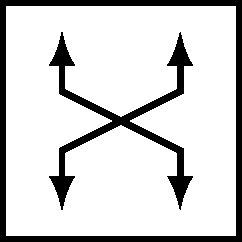
\includegraphics[width=0.9cm]{../common/fig-switch.pdf}
}
\providecommand{\router}{%
    
\includegraphics[width=0.9cm]{../common/fig-router.pdf}
}

\begin{frame}
\frametitle{exercise (1)}
\begin{tikzpicture}
\tikzset{
    computer/.style={inner sep=0mm,outer sep=0mm,execute at begin node={\computer}},
    switch/.style={inner sep=0mm,outer sep=0mm,execute at begin node={\switch}},
    router/.style={inner sep=-1mm,outer sep=0mm,execute at begin node={\router},circle},
    connect/.style={draw,very thick,Latex-Latex},
    connect big/.style={draw,ultra thick,Latex-Latex},
    addr label/.style={align=left,font=\fontsize{9}{10}\selectfont\tt},
}
\node[computer,label={[addr label]south:MAC 00:\ldots:AA\\IP 192.0.2.4}] (n1-c1) at (0, -1.5) {};
\node[computer,label={[addr label]south:MAC 04:\ldots:BB\\IP 192.0.2.5}]  (n1-c2) at (0, 1) {};
\node[switch] (n1-s1) at (3,-1) {};
\draw[connect] (n1-c1) -- (n1-s1);
\draw[connect] (n1-c2) -- (n1-s1);
\node[router,label={[addr label]south:MAC 02:\ldots:DD / 02:\ldots:DE / 02:\ldots:DF\\IP: 192.0.2.1 / 23.0.113.199 / 195.51.100.1}] (n1n2) at (5.5, -2) {};
\node[switch] (n2-s1) at (7, 0) {};
\node[computer,label={[addr label]south:MAC 03:\ldots:EE\\IP: 195.51.100.4}] (n2-c1) at (10, -1) {};
\draw[connect](n2-s1) -- (n2-c1);

\draw[connect big] (n1-s1) -- (n1n2);
\draw[connect big] (n2-s1) -- (n1n2);
    \node[draw,cloud,aspect=2] (internet) at (5, 1) {internet};
    \draw[connect big] (n1n2) -- (internet);
\end{tikzpicture}
\begin{itemize}
\item if no one's neighbor tables are setup yet,
        how many frames get sent when 192.0.2.5 sends one IP packet to 195.51.100.4?
\end{itemize}
\end{frame}


\begin{frame}
\frametitle{exercise (2)}
\begin{tikzpicture}
\tikzset{
    computer/.style={inner sep=0mm,outer sep=0mm,execute at begin node={\computer}},
    switch/.style={inner sep=0mm,outer sep=0mm,execute at begin node={\switch}},
    router/.style={inner sep=-1mm,outer sep=0mm,execute at begin node={\router},circle},
    connect/.style={draw,very thick,Latex-Latex},
    connect big/.style={draw,ultra thick,Latex-Latex},
    addr label/.style={align=left,font=\fontsize{9}{10}\selectfont\tt},
}
\node[computer,label={[addr label]south:MAC 00:\ldots:AA\\IP 192.0.2.4}] (n1-c1) at (0, -1.5) {};
\node[computer,label={[addr label]south:MAC 04:\ldots:BB\\IP 192.0.2.5}]  (n1-c2) at (0, 1) {};
\node[switch] (n1-s1) at (3,-1) {};
\draw[connect] (n1-c1) -- (n1-s1);
\draw[connect] (n1-c2) -- (n1-s1);
\node[router,label={[addr label]south:MAC 02:\ldots:DD / 02:\ldots:DE / 02:\ldots:DF\\IP: 192.0.2.1 / 23.0.113.199 / 195.51.100.1}] (n1n2) at (5.5, -2) {};
\node[switch] (n2-s1) at (7, 0) {};
\node[computer,label={[addr label]south:MAC 03:\ldots:EE\\IP: 195.51.100.4}] (n2-c1) at (10, -1) {};
\draw[connect](n2-s1) -- (n2-c1);

\draw[connect big] (n1-s1) -- (n1n2);
\draw[connect big] (n2-s1) -- (n1n2);
    \node[draw,cloud,aspect=2] (internet) at (5, 1) {internet};
    \draw[connect big] (n1n2) -- (internet);
\begin{visibleenv}<2->
\node[font=\fontsize{11}{12}\selectfont,anchor=north west, overlay] at (8, 2) {%
    \begin{tabular}{|l|l|l|} \hline
    IP addresses & gateway & interface \\\hline
    & & \\
    & & \\
    & & \\
    & & \\
        \hline
    \end{tabular}
};
\end{visibleenv}
\end{tikzpicture}
\begin{itemize}
\item what should 192.0.2.5's routing table look like? How about the router's routing table?
\end{itemize}
\end{frame}

